\documentclass[11pt,a4paper]{article}

% ── Encoding & fonts ─────────────────────────────────────────────────────────
\usepackage[T1]{fontenc}
\usepackage[utf8]{inputenc}
\usepackage{palatino}
\usepackage[scaled=0.92]{helvet}
\usepackage{microtype}

% ── Page geometry ─────────────────────────────────────────────────────────────
\usepackage[top=2.5cm, bottom=2.5cm, left=2.8cm, right=2.8cm]{geometry}

% ── Colours ───────────────────────────────────────────────────────────────────
\usepackage[dvipsnames,svgnames,x11names]{xcolor}
\definecolor{PurpleLight}{HTML}{EEEDFE}
\definecolor{PurpleMid}{HTML}{534AB7}
\definecolor{PurpleDark}{HTML}{3C3489}
\definecolor{TealLight}{HTML}{E1F5EE}
\definecolor{TealMid}{HTML}{0F6E56}
\definecolor{TealDark}{HTML}{085041}
\definecolor{AmberLight}{HTML}{FAEEDA}
\definecolor{AmberMid}{HTML}{854F0B}
\definecolor{CoralLight}{HTML}{FAECE7}
\definecolor{CoralMid}{HTML}{993C1D}
\definecolor{GrayLight}{HTML}{F1EFE8}
\definecolor{GrayMid}{HTML}{5F5E5A}
\definecolor{BlueLight}{HTML}{E6F1FB}
\definecolor{BlueMid}{HTML}{185FA5}
\definecolor{GreenLight}{HTML}{EAF3DE}
\definecolor{GreenMid}{HTML}{3B6D11}
\definecolor{GreenDark}{HTML}{27500A}
\definecolor{InlineCodeBg}{HTML}{F3F2EE}
\definecolor{CodeBg}{HTML}{F7F6F2}
\definecolor{RuleLine}{HTML}{D3D1C7}

% ── Graphics & TikZ ───────────────────────────────────────────────────────────
\usepackage{tikz}
\usetikzlibrary{shapes.geometric, arrows.meta, positioning, fit, backgrounds, decorations.pathreplacing}
\tikzset{
  base node/.style={
    rectangle, rounded corners=4pt, minimum height=1.1cm,
    align=center, font=\small\sffamily, text width=#1,
    inner sep=6pt, draw, thick
  },
  purple node/.style={base node=#1, fill=PurpleLight, draw=PurpleMid, text=PurpleDark},
  teal node/.style={base node=#1, fill=TealLight, draw=TealMid, text=TealDark},
  amber node/.style={base node=#1, fill=AmberLight, draw=AmberMid, text=AmberMid},
  coral node/.style={base node=#1, fill=CoralLight, draw=CoralMid, text=CoralMid},
  gray node/.style={base node=#1, fill=GrayLight, draw=GrayMid, text=GrayMid},
  blue node/.style={base node=#1, fill=BlueLight, draw=BlueMid, text=BlueMid},
  green node/.style={base node=#1, fill=GreenLight, draw=GreenMid, text=GreenDark},
  container/.style={
    rectangle, rounded corners=8pt, dashed, thick,
    inner sep=10pt, fill opacity=0.08, fill=#1, draw=#1
  },
  arrow/.style={-{Stealth[length=6pt]}, thick, color=GrayMid},
  darrow/.style={-{Stealth[length=6pt]}, thick, color=GrayMid, dashed},
}

% ── Code listings ─────────────────────────────────────────────────────────────
\usepackage{listings}
\lstdefinestyle{python}{
  language=Python,
  basicstyle=\ttfamily\small,
  backgroundcolor=\color{CodeBg},
  keywordstyle=\color{PurpleMid}\bfseries,
  commentstyle=\color{GrayMid}\itshape,
  stringstyle=\color{TealMid},
  numberstyle=\tiny\color{GrayMid},
  numbers=left, numbersep=8pt,
  breaklines=true, breakatwhitespace=true,
  frame=single, framerule=0.4pt, rulecolor=\color{RuleLine},
  xleftmargin=14pt, framexleftmargin=14pt,
  showstringspaces=false,
  tabsize=4,
  morekeywords={dataclass, field, Optional, List, dict, str, bool, int, float},
}
\lstdefinestyle{bash}{
  language=bash,
  basicstyle=\ttfamily\small,
  backgroundcolor=\color{CodeBg},
  keywordstyle=\color{TealMid}\bfseries,
  commentstyle=\color{GrayMid}\itshape,
  frame=single, framerule=0.4pt, rulecolor=\color{RuleLine},
  xleftmargin=14pt, framexleftmargin=14pt,
  breaklines=true,
  showstringspaces=false,
}
\lstset{style=python}

% ── Inline code box ───────────────────────────────────────────────────────────
\usepackage{tcolorbox}
\tcbuselibrary{skins, breakable}
\newtcbox{\codebox}{
  nobeforeafter, colback=InlineCodeBg, colframe=RuleLine,
  boxrule=0.4pt, arc=2pt, left=2pt, right=2pt, top=1pt, bottom=1pt,
  fontupper=\ttfamily\small
}
\newcommand{\py}[1]{\codebox{#1}}

% ── Note / warning boxes ──────────────────────────────────────────────────────
\newtcolorbox{notebox}[1][Note]{
  breakable, colback=TealLight, colframe=TealMid,
  boxrule=0.6pt, arc=4pt, left=8pt, right=8pt, top=6pt, bottom=6pt,
  fonttitle=\sffamily\bfseries\small, title=#1, coltitle=white
}
\newtcolorbox{warnbox}[1][Important]{
  breakable, colback=AmberLight, colframe=AmberMid,
  boxrule=0.6pt, arc=4pt, left=8pt, right=8pt, top=6pt, bottom=6pt,
  fonttitle=\sffamily\bfseries\small, title=#1, coltitle=AmberMid
}

% ── Tables ────────────────────────────────────────────────────────────────────
\usepackage{booktabs}
\usepackage{array}
\usepackage{tabularx}
\renewcommand{\arraystretch}{1.3}

% ── Section headings ──────────────────────────────────────────────────────────
\usepackage{titlesec}
\titleformat{\section}{\Large\sffamily\bfseries\color{PurpleDark}}{}{0em}{}[\vspace{-0.5ex}\color{PurpleMid}\rule{\linewidth}{0.8pt}]
\titleformat{\subsection}{\large\sffamily\bfseries\color{TealDark}}{}{0em}{}
\titleformat{\subsubsection}{\normalsize\sffamily\bfseries\color{GrayMid}}{}{0em}{}

% ── TOC & hyperlinks ─────────────────────────────────────────────────────────
\usepackage[hidelinks, colorlinks=true,
  linkcolor=PurpleDark, urlcolor=BlueMid, citecolor=TealMid]{hyperref}
\usepackage{tocloft}
\renewcommand{\cftsecfont}{\sffamily}
\renewcommand{\cftsubsecfont}{\sffamily\small}

% ── Misc ──────────────────────────────────────────────────────────────────────
\usepackage{parskip}
\usepackage{enumitem}
\usepackage{fancyhdr}
\usepackage{amsmath}
\usepackage{caption}
\captionsetup{font=small, labelfont={bf,sf}, labelsep=period}

\pagestyle{fancy}
\fancyhf{}
\fancyhead[L]{\small\sffamily\color{GrayMid} ON-DEM WG3 — YADE Export/Import Pipeline}
\fancyhead[R]{\small\sffamily\color{GrayMid} \leftmark}
\fancyfoot[C]{\small\sffamily\color{GrayMid}\thepage}
\renewcommand{\headrulewidth}{0.3pt}
\renewcommand{\headrule}{\color{RuleLine}\hrule width\headwidth height\headrulewidth}

% =============================================================================
\begin{document}


% ── Title page ────────────────────────────────────────────────────────────────
\begin{titlepage}
\centering
\vspace*{2cm}

{\color{PurpleMid}\rule{\linewidth}{1.5pt}}
\vspace{0.4cm}

{\Huge\sffamily\bfseries\color{PurpleDark} ON-DEM WG3}\\[0.4em]
{\LARGE\sffamily\color{TealDark} YADE $\leftrightarrow$ VTKHDF Export/Import Pipeline}\\[0.3em]
{\large\sffamily\color{GrayMid} Documentation \& Developer Guide — v0.1}

\vspace{0.4cm}
{\color{PurpleMid}\rule{\linewidth}{1.5pt}}
\vspace{1.5cm}

\begin{tcolorbox}[colback=PurpleLight, colframe=PurpleMid, arc=6pt,
  boxrule=0.6pt, width=0.82\textwidth]
\centering\sffamily\small\color{PurpleDark}
\textbf{Proof of concept:} This toolchain was developed for YADE DEM, but the
architecture is intentionally simulator-agnostic. Only a single JSON mapping
file and a small set of helper functions need to be replaced to retarget the
pipeline to any other DEM code (MercuryDPM, LIGGGHTS, EDEM, \ldots).
\end{tcolorbox}

\vspace{1.5cm}

\begin{tabular}{ll}
\toprule
\sffamily\textbf{Authors}          & Bruno Chareyre (\href{mailto:bruno.chareyre@3sr-grenoble.fr}{bruno.chareyre@3sr-grenoble.fr}) \\
                                   & Adrian Priceputu (\href{mailto:adrian.priceputu@utcb.ro}{adrian.priceputu@utcb.ro}) \\
\sffamily\textbf{Working group}    & ON-DEM WG3 \\
\sffamily\textbf{Status}           & Draft v0.1 \\
\sffamily\textbf{Schema version}   & 0.1-draft \\
\sffamily\textbf{Target simulators}& YADE (primary); others planned \\
\bottomrule
\end{tabular}



\vfill
\begin{tcolorbox}[colback=GrayLight, colframe=RuleLine, arc=4pt, boxrule=0.4pt]
\centering\small\sffamily\color{GrayMid}
\textbf{Disclaimer:} Parts of this work, including code and documentation, were
developed with the assistance of AI tools. All content has been reviewed and
validated by the authors.
\end{tcolorbox}

\end{titlepage}

% ── Table of contents ────────────────────────────────────────────────────────
\tableofcontents
\clearpage

% =============================================================================
\section{Overview}
\label{sec:overview}
% =============================================================================

This document describes the ON-DEM WG3 toolchain for exporting and importing
DEM simulation state between YADE and the VTKHDF file format. The pipeline
now supports a complete round-trip: a simulation running in YADE can be
checkpointed to a \texttt{.vtkhdf} file and later resumed — either in YADE
itself or in any other VTK-aware DEM code such as MercuryDPM.

The pipeline consists of seven files:

\begin{table}[htbp]
\centering
\begin{tabular}{llll}
\toprule
\sffamily\textbf{File} & \sffamily\textbf{Role} & \sffamily\textbf{When run} \\
\midrule
\texttt{schema/*.py}                    & ON-DEM field definitions      & never directly \\
\texttt{schema\_parser.py}              & AST reader, Schema builder    & offline, by codegen \\
\texttt{yade\_mapping.json}             & YADE API translation table    & offline, by codegen \\
\texttt{codegen\_dem.py}                & Exporter code generator       & offline, once \\
\texttt{hdf5\_utils.py}                 & Generic HDF5 I/O helpers      & at runtime \\
\texttt{export\_yade\_vtkhdf.py}        & Generated YADE exporter       & at runtime \\
\texttt{import\_yade\_vtkhdf.py}        & YADE importer (round-trip)    & at runtime \\
\bottomrule
\end{tabular}
\caption{Files comprising the ON-DEM export/import pipeline.}
\end{table}

The key design principle is the \textbf{separation of concerns}: the
ON-DEM schema describes physics concepts in simulator-neutral Python classes;
the mapping JSON is the only file that knows anything about YADE's API; and
the code generator bridges the two by emitting a ready-to-run exporter.
All low-level HDF5 read/write logic is centralised in the simulator-agnostic
\texttt{hdf5\_utils.py}, making the generated code clean and the I/O layer
reusable by both the exporter and importer.

% =============================================================================
\section{Architecture and data flow}
\label{sec:architecture}
% =============================================================================

Figure~\ref{fig:pipeline} shows the complete pipeline, now including the
import path that closes the round-trip.

\begin{figure}[h!]
\centering
\resizebox{\linewidth}{!}{%
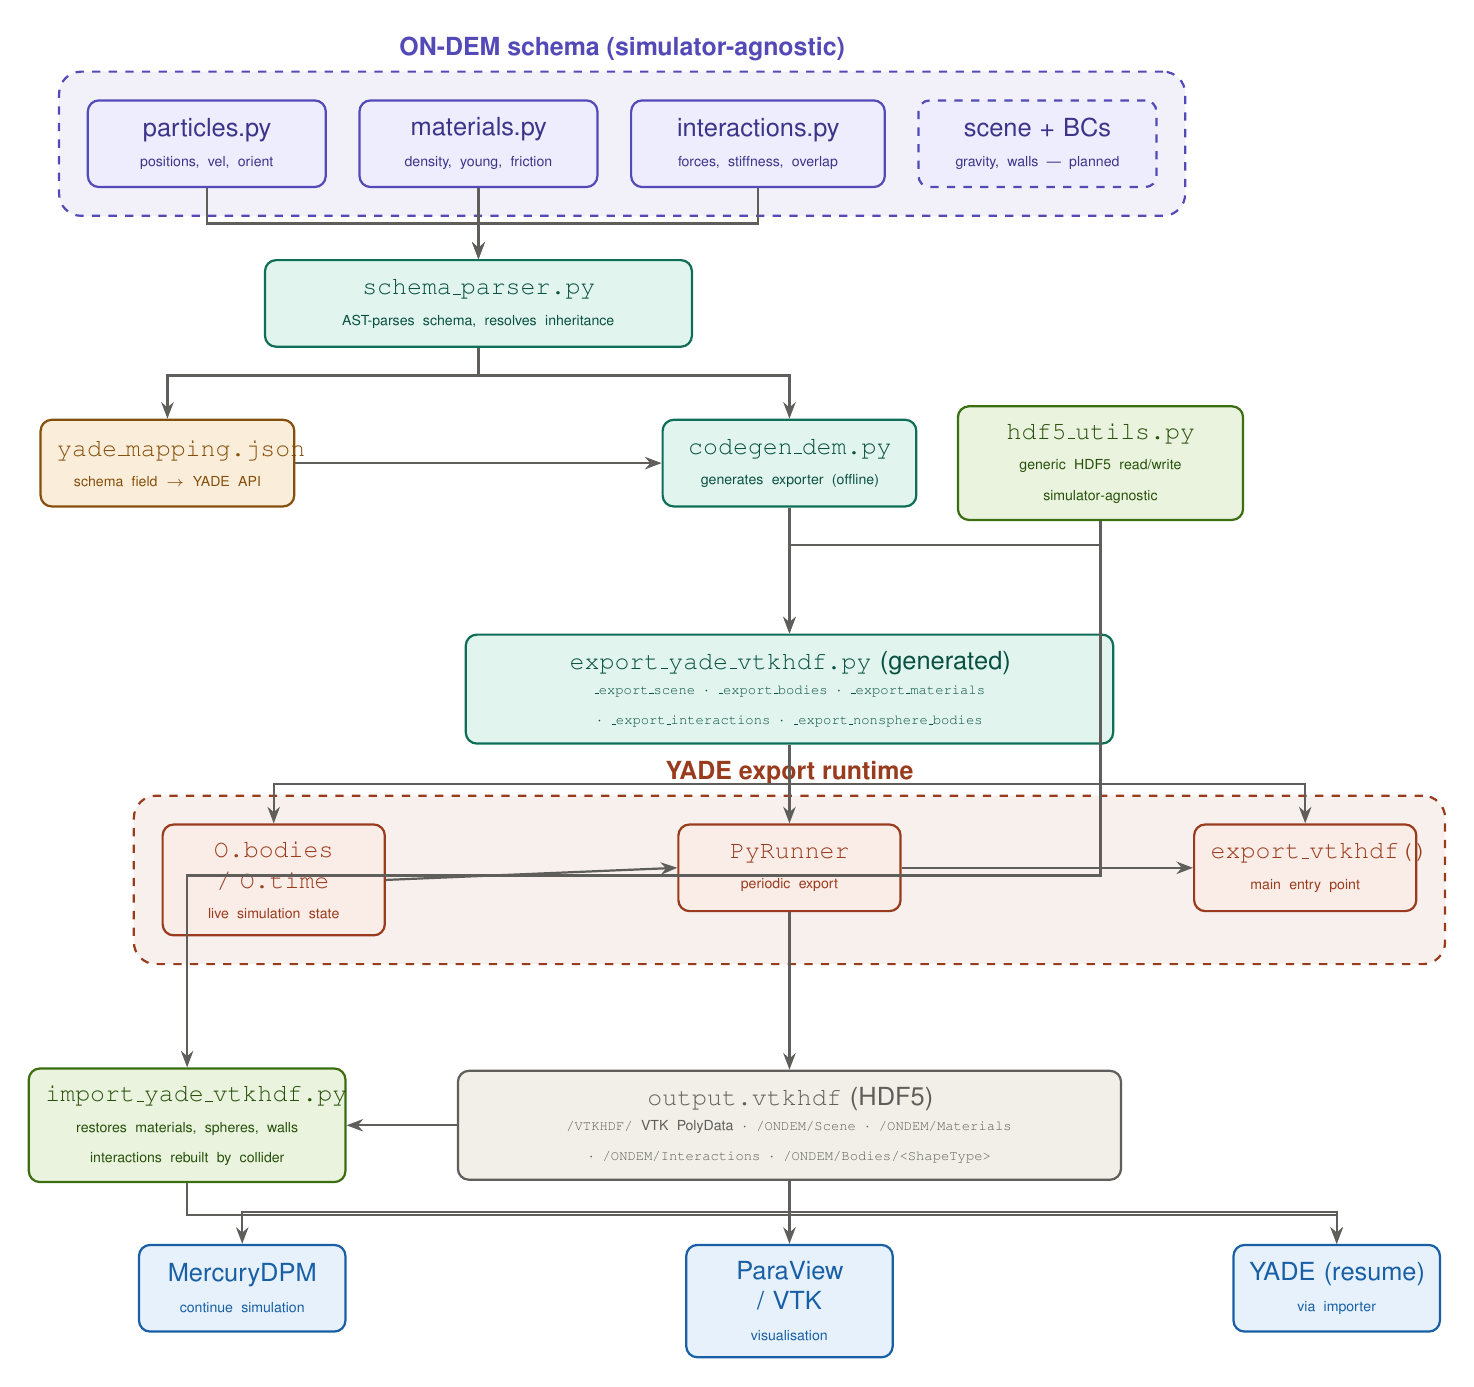
\begin{tikzpicture}[node distance=0.55cm and 0.5cm]

  % ── Layer 0: ON-DEM schema ────────────────────────────────────────────────
  \node[purple node=2.6cm] (particles)   {particles.py\\{\tiny positions, vel, orient}};
  \node[purple node=2.6cm, right=0.4cm of particles] (materials) {materials.py\\{\tiny density, young, friction}};
  \node[purple node=2.8cm, right=0.4cm of materials] (intrs) {interactions.py\\{\tiny forces, stiffness, overlap}};
  \node[purple node=2.6cm, right=0.4cm of intrs, dashed, draw=PurpleMid] (bcs) {scene + BCs\\{\tiny gravity, walls — planned}};

  \begin{scope}[on background layer]
    \node[container=PurpleMid, fit=(particles)(materials)(intrs)(bcs),
          label={[font=\small\sffamily\bfseries\color{PurpleMid}]above:ON-DEM schema (simulator-agnostic)}] {};
  \end{scope}

  % ── schema_parser + mapping + codegen ─────────────────────────────────────
  \node[teal node=5.0cm, below=0.9cm of materials] (parser)
    {\texttt{schema\_parser.py}\\{\tiny AST-parses schema, resolves inheritance}};

  \node[amber node=2.8cm, below left=0.9cm and -0.4cm of parser] (mapping)
    {\texttt{yade\_mapping.json}\\{\tiny schema field $\rightarrow$ YADE API}};

  \node[teal node=2.8cm, below right=0.9cm and -0.4cm of parser] (codegen)
    {\texttt{codegen\_dem.py}\\{\tiny generates exporter (offline)}};

  % ── hdf5_utils ────────────────────────────────────────────────────────────
  \node[green node=3.2cm, right=0.5cm of codegen] (hdf5utils)
    {\texttt{hdf5\_utils.py}\\{\tiny generic HDF5 read/write}\\{\tiny simulator-agnostic}};

  % ── generated exporter ────────────────────────────────────────────────────
  \node[teal node=7.8cm, below=1.6cm of codegen] (exporter)
    {\texttt{export\_yade\_vtkhdf.py} (generated)\\[-2pt]
     {\tiny \texttt{\_export\_scene} $\cdot$ \texttt{\_export\_bodies} $\cdot$ \texttt{\_export\_materials} $\cdot$ \texttt{\_export\_interactions} $\cdot$ \texttt{\_export\_nonsphere\_bodies}}};

  % ── YADE runtime ──────────────────────────────────────────────────────────
  \node[coral node=2.4cm, below left=1.0cm and 1.0cm of exporter] (yadebodies)
    {\texttt{O.bodies / O.time}\\{\tiny live simulation state}};
  \node[coral node=2.4cm, below=1.0cm of exporter] (pyrunner)
    {\texttt{PyRunner}\\{\tiny periodic export}};
  \node[coral node=2.4cm, below right=1.0cm and 1.0cm of exporter] (entrypoint)
    {\texttt{export\_vtkhdf()}\\{\tiny main entry point}};

  \begin{scope}[on background layer]
    \node[container=CoralMid, fit=(yadebodies)(pyrunner)(entrypoint),
          label={[font=\small\sffamily\bfseries\color{CoralMid}]above:YADE export runtime}] {};
  \end{scope}

  % ── Output file ───────────────────────────────────────────────────────────
  \node[gray node=8.0cm, below=2.0cm of pyrunner] (output)
    {\texttt{output.vtkhdf} (HDF5)\\[-2pt]
     {\tiny \texttt{/VTKHDF/} VTK PolyData $\cdot$ \texttt{/ONDEM/Scene} $\cdot$ \texttt{/ONDEM/Materials} $\cdot$ \texttt{/ONDEM/Interactions} $\cdot$ \texttt{/ONDEM/Bodies/<ShapeType>}}};

  % ── Importer (new) ────────────────────────────────────────────────────────
  \node[green node=3.6cm, left=1.4cm of output] (importer)
    {\texttt{import\_yade\_vtkhdf.py}\\{\tiny restores materials, spheres, walls}\\{\tiny interactions rebuilt by collider}};

  % ── Downstream ────────────────────────────────────────────────────────────
  \node[blue node=2.2cm, below left=0.8cm and 1.4cm of output] (mercury)
    {MercuryDPM\\{\tiny continue simulation}};
  \node[blue node=2.2cm, below=0.8cm of output] (paraview)
    {ParaView / VTK\\{\tiny visualisation}};
  \node[blue node=2.2cm, below right=0.8cm and 1.4cm of output] (yaderesume)
    {YADE (resume)\\{\tiny via importer}};

  % ── Arrows ────────────────────────────────────────────────────────────────
  \draw[arrow] (particles.south)  -- ++(0,-0.45) -| (parser.north);
  \draw[arrow] (materials.south)  -- (parser.north);
  \draw[arrow] (intrs.south)      -- ++(0,-0.45) -| (parser.north);
  \draw[arrow] (parser.south)     -- ++(0,-0.35) -| (mapping.north);
  \draw[arrow] (parser.south)     -- ++(0,-0.35) -| (codegen.north);
  \draw[arrow] (mapping.east)     -- (codegen.west);
  \draw[arrow] (codegen.south)    -- ++(0,-0.4) -| (exporter.north);
  \draw[arrow] (hdf5utils.south)  -- ++(0,-0.3) -| (exporter.north);
  \draw[arrow] (exporter.south)   -- ++(0,-0.5) -| (yadebodies.north);
  \draw[arrow] (exporter.south)   -- (pyrunner.north);
  \draw[arrow] (exporter.south)   -- ++(0,-0.5) -| (entrypoint.north);
  \draw[arrow] (yadebodies.east)  -- (pyrunner.west);
  \draw[arrow] (pyrunner.east)    -- (entrypoint.west);
  \draw[arrow] (pyrunner.south)   -- ++(0,-0.35) -- (output.north);
  \draw[arrow] (hdf5utils.south)  -- ++(0,-4.5) -| (importer.north);
  \draw[arrow] (output.west)      -- (importer.east);
  \draw[arrow] (output.south)     -- ++(0,-0.4) -| (mercury.north);
  \draw[arrow] (output.south)     -- (paraview.north);
  \draw[arrow] (output.south)     -- ++(0,-0.4) -| (yaderesume.north);
  \draw[arrow] (importer.south)   -- ++(0,-0.4) -| (yaderesume.north);

\end{tikzpicture}}
\caption{Complete ON-DEM export/import pipeline. The round-trip YADE $\rightarrow$ VTKHDF $\rightarrow$ YADE is fully supported. \texttt{hdf5\_utils.py} is shared by both the exporter and importer.}
\label{fig:pipeline}
\end{figure}

\begin{notebox}[Generality by design]
The only YADE-specific artefacts are \texttt{yade\_mapping.json} and the
helper functions (\texttt{\_get\_gravity}, \texttt{\_sphere\_volume}, etc.)
in the generated exporter. The schema files, \texttt{schema\_parser.py},
\texttt{codegen\_dem.py}, and \texttt{hdf5\_utils.py} are all
simulator-neutral. Retargeting to MercuryDPM or LIGGGHTS requires only a
new mapping JSON and a matching importer.
\end{notebox}

% =============================================================================
\section{\texttt{schema\_parser.py} --- the schema reader}
\label{sec:schema_parser}
% =============================================================================

\texttt{schema\_parser.py} is a pure offline utility. It reads the ON-DEM
schema \texttt{.py} files using Python's \texttt{ast} module (without
importing them), builds an in-memory structured representation of every class
and field, and returns a \texttt{Schema} object consumed by the code
generator.

\subsection{Three-phase execution}

The script executes in three sequential phases:

\begin{enumerate}[leftmargin=1.8em, itemsep=4pt]
  \item \textbf{File parsing} --- \py{\_parse\_file()} is called once per
    \texttt{.py} file. It uses \texttt{ast.parse()} to obtain a syntax tree,
    walks it for \py{ClassDef} nodes, and for each class extracts field
    names, type annotations, default values, and docstrings via a lookahead
    on the next statement in the class body.
  \item \textbf{Inheritance resolution} --- \py{\_resolve\_inheritance()}
    fills \py{all\_fields} on each \py{ClassDef} by recursively walking base
    classes and merging ancestor fields with own fields (child overrides
    parent on name clash).
  \item \textbf{Schema assembly} --- all \py{ClassDef} objects are collected
    into a \py{Schema} dataclass and returned.
\end{enumerate}

\subsection{Type inference}

The \py{\_infer\_hdf5()} function maps Python type annotations to HDF5
storage types and array shapes:

\begin{table}[htbp]
\centering
\begin{tabular}{lll}
\toprule
\sffamily\textbf{Python type} & \sffamily\textbf{HDF5 type} & \sffamily\textbf{Array shape} \\
\midrule
\texttt{float}      & \texttt{scalar\_float}  & \texttt{scalar} \\
\texttt{int}        & \texttt{scalar\_int}    & \texttt{scalar} \\
\texttt{bool}       & \texttt{scalar\_bool}   & \texttt{scalar} \\
\texttt{str}        & \texttt{string}         & \texttt{scalar} \\
\texttt{Vector3}    & \texttt{vector3}        & \texttt{(N,3)}  \\
\texttt{Quaternion} & \texttt{quaternion}     & \texttt{(N,4)}  \\
\texttt{Matrix3}    & \texttt{matrix3}        & \texttt{(N,9)}  \\
\texttt{List[str]}  & \texttt{string\_list}   & \texttt{(N,)}   \\
\bottomrule
\end{tabular}
\caption{Mapping from Python type annotations to HDF5 types and array shapes.}
\end{table}

\begin{warnbox}[Known issue: type inference for schema base types]
When \texttt{base\_types.py} is skipped (as intended), the type annotations
in the schema files refer to names like \texttt{Vector3} and \texttt{float}
that the AST parser never sees defined. In the current version,
\texttt{ast.unparse()} on these annotation nodes can return an AST object
representation string (e.g.\ \texttt{<\_ast.Name object at 0x...>}) instead
of the clean type name. This causes \texttt{hdf5\_type} to be set to
\texttt{"unknown"} for affected fields. These fields are still exported
correctly because \texttt{hdf5\_utils.hdf5\_write\_field()} handles the
\texttt{"unknown"} case gracefully, but the generated code comments show the
raw AST repr. This will be fixed in a future version.
\end{warnbox}

\subsection{Public API}

\begin{lstlisting}
from schema_parser import parse_schema_dir

schema = parse_schema_dir("/path/to/schema/")
# schema.classes  -> dict[str, ClassDef]
# schema.modules  -> dict[str, list[str]]
\end{lstlisting}

Files named \texttt{base\_types.py} and \texttt{model.py} are skipped
automatically.

% =============================================================================
\section{\texttt{yade\_mapping.json} --- the translation layer}
\label{sec:mapping}
% =============================================================================

This JSON file is the \emph{only simulator-specific file} in the offline
pipeline. It maps each ON-DEM schema field name to the YADE Python expression
that reads it at simulation runtime.

\subsection{Structure}

\begin{lstlisting}[language={}]
{
  "scene": {
    "time":     "O.time",
    "timestep": "O.dt",
    "gravity":  "_get_gravity()"
  },
  "state": {
    "position":         "b.state.pos",
    "velocity":         "b.state.vel",
    "orientation":      "b.state.ori",
    "angular_velocity": "b.state.angVel",
    "mass":             "b.state.mass"
  },
  "normal": {
    "normal_force": "(i.phys.normalForce.norm() *
      (1.0 if i.phys.normalForce.dot(i.geom.normal) >= 0 else -1.0))"
  }
  ...
}
\end{lstlisting}

Keys prefixed with \texttt{\_} contain fields that go beyond the ON-DEM
schema but are exported for interoperability (geometry data, material labels,
physics type strings).

\subsection{Retargeting to a different simulator}

Create a new mapping file with the same key structure but expressions from
the target simulator's Python API, then regenerate:

\begin{lstlisting}[style=bash]
python codegen_dem.py schema/ \
    --mapping mercury_mapping.json \
    --out export_mercury_vtkhdf.py
\end{lstlisting}

% =============================================================================
\section{\texttt{hdf5\_utils.py} --- the generic I/O layer}
\label{sec:hdf5utils}
% =============================================================================

\texttt{hdf5\_utils.py} is a simulator-agnostic module that centralises
all HDF5 read and write operations. Both the generated exporter and the
importer import from it, avoiding duplicated low-level NumPy/h5py code.

\subsection{Write functions}

\begin{table}[htbp]
\centering
\begin{tabularx}{\textwidth}{>{\ttfamily\small\raggedright\arraybackslash}p{0.60\linewidth}>{\small\raggedright\arraybackslash}p{0.35\linewidth}}
\toprule
\sffamily\textbf{Function} & \sffamily\textbf{Purpose} \\
\midrule
hdf5\_write\_field(grp, name, hdf5\_type, value, scalar\_as\_dataset) &
  Write a single field (type dispatcher) \\
hdf5\_write\_scalar\_array(grp, name, values, dtype) &
  Write 1-D array of scalars \\
hdf5\_write\_vector3\_array(grp, name, values) &
  Write $(N,3)$ float64 array \\
hdf5\_write\_quaternion\_array(grp, name, values) &
  Write $(N,4)$; reorders $w,x,y,z \to x,y,z,w$ \\
hdf5\_write\_matrix3\_array(grp, name, values) &
  Write $(N,9)$ row-major float64 \\
hdf5\_write\_string\_array(grp, name, values) &
  Write variable-length string dataset \\
\bottomrule
\end{tabularx}
\caption{HDF5 write utility functions in \texttt{hdf5\_utils.py}.}
\end{table}

\subsection{Read functions}

\begin{table}[htbp]
\centering
\begin{tabularx}{\textwidth}{>{\ttfamily\small\raggedright\arraybackslash}p{0.60\linewidth}>{\small\raggedright\arraybackslash}p{0.35\linewidth}}
\toprule
\sffamily\textbf{Function} & \sffamily\textbf{Purpose} \\
\midrule
hdf5\_read\_field(grp, name, hdf5\_type, scalar\_as\_dataset) &
  Read a single field (type dispatcher) \\
hdf5\_read\_scalar\_array(grp, name, dtype) &
  Read 1-D array of scalars \\
hdf5\_read\_vector3\_array(grp, name) &
  Read $(N,3)$; returns list of lists \\
hdf5\_read\_quaternion\_array(grp, name) &
  Read $(N,4)$; reverses to YADE $[w,x,y,z]$ \\
hdf5\_read\_string\_array(grp, name) &
  Read variable-length strings, decoding bytes \\
\bottomrule
\end{tabularx}
\caption{HDF5 read utility functions in \texttt{hdf5\_utils.py}.}
\end{table}

\subsection{Quaternion convention}

\begin{warnbox}[Quaternion storage convention]
YADE stores quaternions as $(w, x, y, z)$ where \texttt{q[0] = w}
(scalar-first). The ON-DEM/VTKHDF convention is $(x, y, z, w)$
(scalar-last). \texttt{hdf5\_utils} handles this automatically in both
directions: write converts $w,x,y,z \to x,y,z,w$; read reverses $x,y,z,w
\to w,x,y,z$.
\end{warnbox}

% =============================================================================
\section{\texttt{codegen\_dem.py} --- the code generator}
\label{sec:codegen}
% =============================================================================

\texttt{codegen\_dem.py} is a simulator-agnostic code generator. It reads
the \texttt{Schema} object and the mapping JSON, then writes a complete
Python exporter as a \texttt{.py} source file.

\subsection{Usage}

\begin{lstlisting}[style=bash]
python codegen_dem.py <schema_dir> \
    [--mapping yade_mapping.json]  \
    [--out export_yade_vtkhdf.py]
\end{lstlisting}

\subsection{Body export: \texttt{\_export\_bodies()}}

\py{\_gen\_bodies\_exporter()} handles all body types in a unified loop:

\begin{itemize}[leftmargin=1.8em, itemsep=2pt]
  \item iterates over all shape types: \texttt{Sphere}, \texttt{Box},
    \texttt{Polyhedron}, \texttt{Wall}, \texttt{Facet};
  \item writes per-body data to \texttt{/ONDEM/Bodies/<ShapeType>/} for
    each type present in the scene;
  \item additionally writes a unified \texttt{/VTKHDF/} PolyData group with
    all body centres as Points and a \texttt{shape\_type} string array in
    PointData, which is what ParaView reads for visualisation.
\end{itemize}

\subsection{Interaction export by physics type}
\py{\_gen\_interactions\_exporter()} groups interactions by their YADE
physics object type (\texttt{FrictPhys}, \texttt{HertzMindlinPhys}, etc.)
and writes each group to \texttt{/ONDEM/Interactions/<PhysType>/}.

\subsection{Generated sections}

\begin{table}[htbp]
\centering
\begin{tabularx}{\textwidth}{>{\ttfamily\small\raggedright\arraybackslash}p{0.38\linewidth}>{\ttfamily\small\raggedright\arraybackslash}p{0.32\linewidth}>{\small\raggedright\arraybackslash}p{0.23\linewidth}}
\toprule
\sffamily\textbf{Generator function} & \sffamily\textbf{Emits} & \sffamily\textbf{Output group} \\
\midrule
\_gen\_header()                 & (imports + docstring)              & top of file \\
\_gen\_helpers()                & \_get\_gravity() etc.              & helper functions \\
\_gen\_scene\_exporter()        & \_export\_scene()                  & \texttt{/ONDEM/Scene} \\
\_gen\_materials\_exporter()    & \_export\_materials()              & \texttt{/ONDEM/Materials} \\
\_gen\_bodies\_exporter()       & \_export\_bodies()                 & \texttt{/ONDEM/Bodies/<Type>} \\
\_gen\_interactions\_exporter() & \_export\_interactions()           & \texttt{/ONDEM/Interactions/<Type>} \\
\_gen\_nonsphere\_exporter()    & \_export\_nonsphere\_bodies()      & \texttt{/ONDEM/Bodies} \\
\_gen\_main\_function()         & export\_vtkhdf()                   & entry point \\
\bottomrule
\end{tabularx}
\caption{Generator functions in \texttt{codegen\_dem.py} and their output.}
\end{table}

% =============================================================================
\section{\texttt{export\_yade\_vtkhdf.py} --- the generated exporter}
\label{sec:exporter}
% =============================================================================

This file is auto-generated by \texttt{codegen\_dem.py} and should not be
edited manually. Re-run the generator whenever the schema or mapping changes.

\subsection{Usage inside YADE}

\begin{lstlisting}
from export_yade_vtkhdf import export_vtkhdf

# Single snapshot
export_vtkhdf("snapshot_000.vtkhdf")

# Periodic export every 1000 iterations
O.engines += [
    PyRunner(
        command='export_vtkhdf("sim_%04d.vtkhdf" % O.iter)',
        iterPeriod=1000
    )
]
\end{lstlisting}

\subsection{Output file structure}

The HDF5 file layout has changed in v0.2. Body data is now separated by
shape type under \texttt{/ONDEM/Bodies/} rather than being stored as VTK
PointData. The \texttt{/VTKHDF/} group is retained for ParaView
compatibility but only holds body centres and a shape-type string array.

\begin{center}
\resizebox{\linewidth}{!}{%
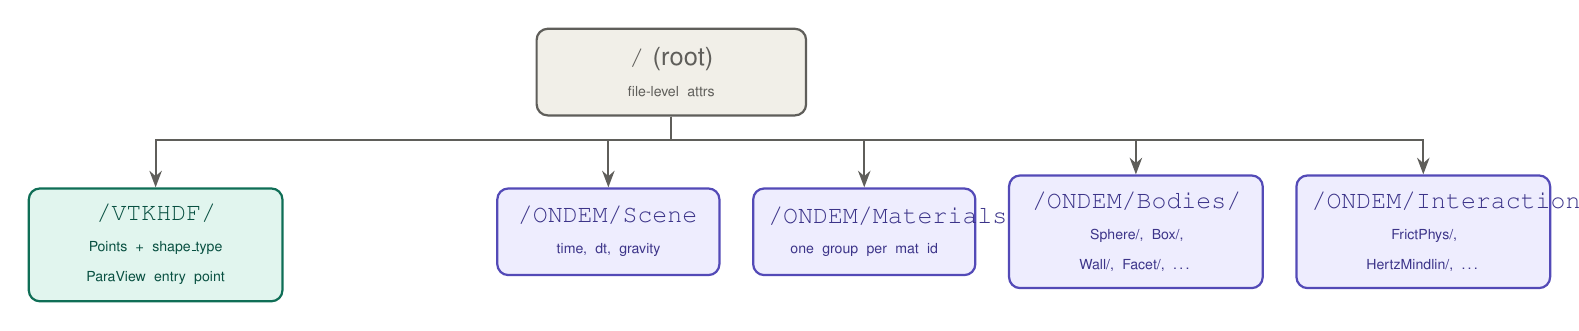
\begin{tikzpicture}
  \node[gray node=3.0cm] (root) {\texttt{/} (root)\\{\tiny file-level attrs}};

  \node[teal node=2.8cm, below left=0.9cm and 3.2cm of root] (vtkhdf)
    {\texttt{/VTKHDF/}\\{\tiny Points + shape\_type}\\{\tiny ParaView entry point}};

  \node[purple node=2.4cm, below=0.9cm of root, xshift=-0.8cm] (scene)
    {\texttt{/ONDEM/Scene}\\{\tiny time, dt, gravity}};

  \node[purple node=2.4cm, right=0.4cm of scene] (mats)
    {\texttt{/ONDEM/Materials}\\{\tiny one group per mat id}};

  \node[purple node=2.8cm, right=0.4cm of mats] (bodies)
    {\texttt{/ONDEM/Bodies/}\\{\tiny Sphere/, Box/,}\\{\tiny Wall/, Facet/, \ldots}};

  \node[purple node=2.8cm, right=0.4cm of bodies] (intrs)
    {\texttt{/ONDEM/Interactions/}\\{\tiny FrictPhys/,}\\{\tiny HertzMindlin/, \ldots}};

  \draw[arrow] (root.south) -- ++(0,-0.3) -| (vtkhdf.north);
  \draw[arrow] (root.south) -- ++(0,-0.3) -| (scene.north);
  \draw[arrow] (root.south) -- ++(0,-0.3) -| (mats.north);
  \draw[arrow] (root.south) -- ++(0,-0.3) -| (bodies.north);
  \draw[arrow] (root.south) -- ++(0,-0.3) -| (intrs.north);
\end{tikzpicture}}
\end{center}

\medskip
\noindent\textbf{\texttt{/VTKHDF/} group.} Contains a VTK PolyData structure
for all bodies. \texttt{Points} holds body centre coordinates; the
\texttt{PointData/shape\_type} string array identifies the shape type of each
body. This group is the entry point for ParaView.

\medskip
\noindent\textbf{\texttt{/ONDEM/Bodies/<ShapeType>/} groups.} One sub-group
per shape type present in the scene (\texttt{Sphere}, \texttt{Box},
\texttt{Wall}, \texttt{Facet}, \texttt{Polyhedron}). Each contains the full
set of per-body arrays (body\_id, material\_id, position, velocity,
orientation, mass, inertia, radius, etc.) for that shape type.

\medskip
\noindent\textbf{\texttt{/ONDEM/Interactions/<PhysType>/} groups.} One
sub-group per YADE physics object type present in the scene. Each contains
contact data: id pairs, normal/shear forces, contact geometry, stiffness
values, and overlap depth.

\medskip
\noindent\textbf{\texttt{/ONDEM/Materials/<id>/} groups.} One sub-group per
unique material ID. Each contains scalar datasets for all material properties
available for that material type. Fields unavailable for a given material are
silently skipped.

\medskip
\noindent\textbf{\texttt{/ONDEM/Scene} group.} Stores \texttt{time} and
\texttt{timestep} as HDF5 attributes, and \texttt{gravity} (3-element float
dataset) and \texttt{units} (string list dataset).

% =============================================================================
\section{\texttt{import\_yade\_vtkhdf.py} --- the importer}
\label{sec:importer}
% =============================================================================

\texttt{import\_yade\_vtkhdf.py} reads a \texttt{.vtkhdf} file written by
the exporter and reconstructs the YADE simulation state: scene metadata,
materials, sphere bodies, and walls.

\subsection{What is restored}

\begin{table}[htbp]
\centering
\begin{tabularx}{\textwidth}{>{\raggedright\arraybackslash}p{0.32\linewidth}>{\ttfamily\small\raggedright\arraybackslash}p{0.35\linewidth}>{\small\raggedright\arraybackslash}X}
\toprule
\sffamily\textbf{Component} & \sffamily\textbf{Source in file} & \sffamily\textbf{Status} \\
\midrule
Time step \texttt{O.dt}   & \texttt{/ONDEM/Scene} attrs     & restored \\
Gravity                    & \texttt{/ONDEM/Scene/gravity}   & restored (needs NewtonIntegrator) \\
Simulated time \texttt{O.time} & \texttt{/ONDEM/Scene} attrs & \emph{read-only in YADE;} printed only \\
Materials (\texttt{FrictMat}) & \texttt{/ONDEM/Materials/}   & restored \\
Sphere bodies              & \texttt{/VTKHDF/PointData/}     & restored \\
Wall bodies                & \texttt{/ONDEM/Bodies/Walls/}   & restored \\
Interactions               & \texttt{/ONDEM/Interactions/}   & \emph{not restored — rebuilt by collider} \\
\bottomrule
\end{tabularx}
\caption{Simulation state components and their restoration status.}
\end{table}

\begin{notebox}[Why interactions are not restored]
Interactions in YADE are ephemeral: they are created and destroyed by the
collision detection algorithm every time step. The correct approach when
resuming a simulation is to let YADE's \texttt{InsertionSortCollider}
regenerate all contacts on the first time step from the restored body
positions. Importing saved interaction data would be fragile and is not
necessary for a correct restart.
\end{notebox}

\begin{warnbox}[\texttt{O.time} is read-only in YADE]
The YADE attribute \texttt{O.time} is a computed property derived from
\texttt{O.iter} and \texttt{O.dt} and cannot be set directly. When a
simulation is resumed via the importer, \texttt{O.iter} resets to~0.
The saved time value is printed to the console for reference but not
applied. If exact time continuity is required, set \texttt{O.iter}
manually before running.
\end{warnbox}

\subsection{Usage}

\begin{lstlisting}
from import_yade_vtkhdf import import_vtkhdf

# Engines must exist before import (so gravity can be applied)
O.engines = [
    ForceResetter(),
    InsertionSortCollider([Bo1_Sphere_Aabb(), Bo1_Wall_Aabb()]),
    InteractionLoop(
        [Ig2_Sphere_Sphere_ScGeom(), Ig2_Wall_Sphere_ScGeom()],
        [Ip2_FrictMat_FrictMat_FrictPhys()],
        [Law2_ScGeom_FrictPhys_CundallStrack()],
    ),
    NewtonIntegrator(gravity=(0, 0, -9.81), damping=0.3),
]

result = import_vtkhdf("sim_0000.vtkhdf")
# result['sphere_ids']  -- list of YADE body ids
# result['wall_ids']    -- list of YADE body ids
# result['mat_id_map']  -- {stored_mat_id -> O.materials index}

O.run(10000, wait=True)
\end{lstlisting}

\subsection{Standalone usage}

\begin{lstlisting}[style=bash]
yade import_yade_vtkhdf.py -- sim_0000.vtkhdf
\end{lstlisting}

The standalone entry point sets up a minimal engine configuration
automatically. Adjust the contact law as needed for your simulation.

\subsection{Internal functions}

\begin{table}[htbp]
\centering
\begin{tabularx}{\textwidth}{>{\ttfamily\small\raggedright\arraybackslash}p{0.60\linewidth}>{\small\raggedright\arraybackslash}p{0.35\linewidth}}
\toprule
\sffamily\textbf{Function} & \sffamily\textbf{Purpose} \\
\midrule
\_read\_scene(f)              & Returns \texttt{(time, dt, gravity)} from \texttt{/ONDEM/Scene} \\
\_read\_materials(f)          & Appends \texttt{FrictMat} objects to \texttt{O.materials} \\
\_read\_spheres(f, mat\_map)  & Appends sphere bodies to \texttt{O.bodies} \\
\_read\_walls(f, mat\_map)    & Appends wall bodies to \texttt{O.bodies} (if present) \\
import\_vtkhdf(filename, ...) & Main entry point; calls all of the above \\
\bottomrule
\end{tabularx}
\caption{Internal functions of \texttt{import\_yade\_vtkhdf.py}.}
\end{table}

% =============================================================================
\section{Extending the pipeline}
\label{sec:extending}
% =============================================================================

\subsection{Adding new schema fields}

Edit the relevant \texttt{schema/*.py} file:

\begin{lstlisting}
class state:
    # existing fields ...
    charge: float = None
    """Electric charge on the particle. [optional] [C]"""
\end{lstlisting}

Add the YADE expression to \texttt{yade\_mapping.json}:

\begin{lstlisting}[language={}]
"state": {
    "charge": "b.state.charge if hasattr(b.state,'charge') else 0.0"
}
\end{lstlisting}

Regenerate the exporter:

\begin{lstlisting}[style=bash]
python codegen_dem.py schema/ --out export_yade_vtkhdf.py
\end{lstlisting}

\subsection{Targeting a different simulator}

\begin{enumerate}[leftmargin=1.8em, itemsep=3pt]
  \item Copy \texttt{yade\_mapping.json} to \texttt{mercury\_mapping.json}.
  \item Replace all YADE API expressions with expressions from the target
    simulator's Python API.
  \item Run: \texttt{python codegen\_dem.py schema/ --mapping mercury\_mapping.json --out export\_mercury\_vtkhdf.py}
  \item Write a matching importer using \texttt{hdf5\_utils} for the I/O
    layer.
\end{enumerate}

The ON-DEM schema files, \texttt{schema\_parser.py}, \texttt{codegen\_dem.py},
and \texttt{hdf5\_utils.py} are reused unchanged.

\subsection{Planned additions to the schema}

\begin{center}
\begin{tabular}{lll}
\toprule
\sffamily\textbf{Schema class} & \sffamily\textbf{Planned fields} & \sffamily\textbf{Status} \\
\midrule
\texttt{scene}        & boundary conditions, domain size   & planned \\
\texttt{body}         & clump membership, fragment ID       & planned \\
\texttt{state}        & charge, liquid film volume          & draft \\
\texttt{interactions} & adhesion force, bond stiffness      & planned \\
\bottomrule
\end{tabular}
\end{center}

% =============================================================================
\section{Dependencies and installation}
\label{sec:deps}
% =============================================================================

\begin{table}[htbp]
\centering
\begin{tabularx}{\textwidth}{>{\ttfamily\small}p{0.12\linewidth}>{\small}p{0.28\linewidth}>{\small}p{0.22\linewidth}>{\small\raggedright\arraybackslash}X}
\toprule
\sffamily\textbf{Package} & \sffamily\textbf{Used by} & \sffamily\textbf{Purpose} & \sffamily\textbf{Install} \\
\midrule
numpy  & exporter, importer, hdf5\_utils & array construction  & \texttt{pip install numpy} \\
h5py   & exporter, importer, hdf5\_utils & HDF5 read/write     & \texttt{pip install h5py} \\
\normalfont YADE & exporter, importer     & simulation runtime  & see YADE docs \\
ast    & schema\_parser                  & schema parsing      & built-in (stdlib) \\
json   & codegen\_dem                    & mapping file        & built-in (stdlib) \\
\bottomrule
\end{tabularx}
\caption{Python package dependencies.}
\end{table}

\begin{notebox}[No VTK dependency on the Python side]
Both the exporter and importer use \texttt{h5py} directly. VTK Python
bindings are not required. VTK is only needed by visualisation tools such as
ParaView, or by a DEM code (e.g.\ MercuryDPM) that uses the VTK reader on
its C++ side.
\end{notebox}

% =============================================================================
\section{Quick reference}
\label{sec:quickref}
% =============================================================================

\begin{table}[htbp]
\centering
\begin{tabularx}{\textwidth}{lX}
\toprule
\sffamily\textbf{Task} & \sffamily\textbf{Command} \\
\midrule
Parse schema only    &
  \texttt{python schema\_parser.py ./schema/} \\[4pt]
Regenerate exporter  &
  \texttt{python codegen\_dem.py schema/ -{}-mapping yade\_mapping.json -{}-out export\_yade\_vtkhdf.py} \\[4pt]
Export from YADE     &
  \texttt{from export\_yade\_vtkhdf import export\_vtkhdf; export\_vtkhdf("out.vtkhdf")} \\[4pt]
Periodic export      &
  \texttt{PyRunner(command='export\_vtkhdf("sim\_\%04d.vtkhdf" \% O.iter)', iterPeriod=1000)} \\[4pt]
Import into YADE     &
  \texttt{from import\_yade\_vtkhdf import import\_vtkhdf; import\_vtkhdf("out.vtkhdf")} \\[4pt]
Standalone import    &
  \texttt{yade import\_yade\_vtkhdf.py -{}- sim\_0000.vtkhdf} \\[4pt]
Inspect output       &
  \texttt{python -c "import h5py; f=h5py.File('out.vtkhdf'); print(list(f.keys()))"} \\
\bottomrule
\end{tabularx}
\caption{Quick reference: common commands.}
\end{table}

\vfill
\begin{tcolorbox}[colback=GrayLight, colframe=RuleLine, arc=4pt, boxrule=0.4pt]
\centering\small\sffamily\color{GrayMid}
ON-DEM WG3 \textbullet\;
Authors: Bruno Chareyre \& Adrian Priceputu \textbullet\;
Documentation draft v0.1 \textbullet\;
Do not edit the generated exporter manually --- re-run \texttt{codegen\_dem.py} to update.
\end{tcolorbox}

\end{document}
